% !TeX root = ../main.tex

\chapter{基于乐观级联锁的模块设计}

索引模块是数据库存储管理模块的重要组成部分。索引模块的设计,同时也需要考虑数据库中整体存储管理模块的设计与实现,
做到二者无缝衔接。接下来的一章,我们将着重介绍基于乐观级联锁的索引模块的设计,同时我们还会介绍当前系统的存储模块与索引
模块交互的部分。

我们将本章分为6个小节逐步介绍ART索引模块。2.1小节主要介绍ART的底层数据结构设计,2.2小节重点介绍了如何基于乐观锁的并发控制
2.3小节介绍了数据库索引模块的内存管理机制,2.4小节介绍索引的操作算法设计,2.5小节主要介绍如何针对不同的数据类型设计相应的Key,
2.6小节介绍了创建和删除索引所需要的事务机制支持,2.7小节介绍了数据库内存表的组织方式,2.8小节对本章内容进行了小结。

\section{ART的底层数据结构}

ART(Adaptive Radix Tree)意为节点可伸缩的前缀树,下面我们将重点介绍这一数据结构的详细设计

\subsection{ART索引节点的头部设计}

\begin{figure}[h]
  \centering
  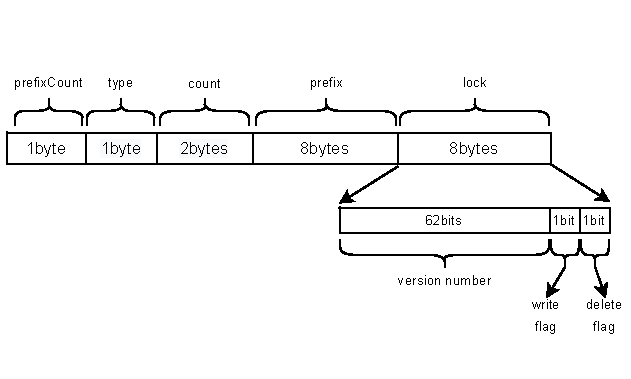
\includegraphics[width=0.9\textwidth]{art-node-design.pdf}
  \caption{ART索引节点的结构图}
  \label{fig:art-node-design}
\end{figure}

与一般前缀树相比,ART最特殊的地方在于内部节点的大小可以根据节点的实际容量而改变。因此我们也需要额外的信息来维护
节点的信息。ART节点分为4种类型,每一种类型的节点都包含一个通用的头部,如下图所示:prefixCount表示公共前缀的长度;
count表示当前节点的子节点个数;optimistic lock用作下文中即将介绍的并发控制机制, 64位原子变量,最后两位分别作为
标记删除和标记修改位;此外由于本索引还需要支持最长前缀匹配,即可能出现某个键值可能是已有键值的前缀,所以还需要加入
isPrefix 和 PrefixSlot 这两个变量分别为标记当前节点是否包含一个额外的子节点和存储子节点的槽位。公共前缀的目的在于
压缩字典树的深度,防止字典树深度过大,造成内存的开销以及访问开销。

\subsection{ART索引各个节点结构定义}

\begin{figure}[h]
  \centering
  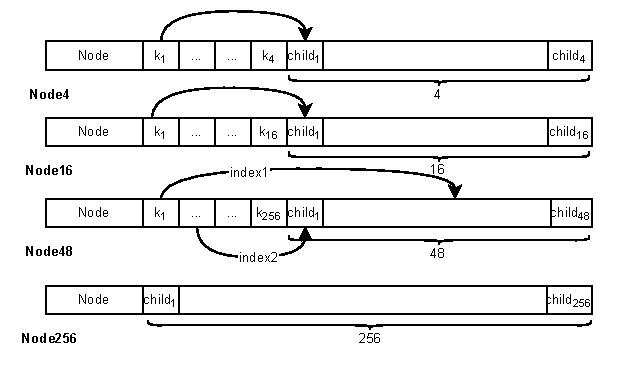
\includegraphics[width=0.9\textwidth]{art-nodes-design.pdf}
  \caption{ART所有类型索引节点的结构图}
  \label{fig:art-nodes-design}
\end{figure}

上面我们已经介绍了所有类型的ART节点都包含的公共头部,下面我们依次介绍每一种节点的设计以及针对每一种节点的优化。
我们按照节点可存储子节点的个数规定四种类型的索引内部节点。依次标记为Node4、Node16、Node48、Node256。下图定义了
四种节点的内存布局。Node4节点keys数组存储键值,children数组存储子节点指针,keys和children一一对应,且keys为
有序数组;Node16节点节点布局和Node4相同只是子节点个数为16,不同的是由于存储个数较多,所以针对节点查询可以利用
SIMD同时比较16个key上的值,后面实现章节会详细说明;Node48节点存储的就是256个key和48个子节点槽位,keys中存储
的是对应在children的索引,即keys[i]与children[keys[i]]对应,无效的keys中存储48即可。Node256节点就是最常规的
前缀树索引的节点。
此外,我们还需要说明所有children中存储的都是指向子节点的指针,由于索引的应用场景为内存数据库,因此使用指针即可
访问对应的子节点。但是同时也引入了一个问题,即如何区分叶子节点?这里我们考虑到实际虚拟内存寻址也仅仅使用低48位内存
地址,所以需要将叶子节点指针的最高位标记为1。

由于本系统需要支持lpm(最长前缀匹配),因此需要针对此需求特殊设计一种ART索引。
因为前缀树本身并不允许一个key是另一个key的前缀,所以可以修改节点的定义,在节点的头部加入一个标记位,
标记当前节点是否作为一个叶节点。
而对于插入删除等索引操作部分的优化,则在接下来的章节部分做出说明。

\section{基于乐观级联锁的并发控制机制}
本论文采用乐观锁来实现ART索引的并发控制。在基于乐观锁的ART索引并发机制中,我们重点关注下面的两个问题:

(1)应当避免某个写操作持有写锁导致其他读写操作多次从根节点重新操作,造成CPU资源的浪费,因此可以在读写操作中加入判断条件即restart次数大于阈值时进程睡眠,让出CPU资源,避免进程被CPU反复无效调度。

(2)同一个进程至多只会同时持有两把写锁,即当前结点和父亲结点。且申请顺序为先申请父亲结点再申请当前结点。且当修改结点的操作完成后应立即释放持有的写锁。索引的插入删除等过程后面具有具体的论述。

我们在每个ART索引节点中都使用一个64位的原子变量作为乐观锁。
当对索引进行操作时,总是先从根节点开始向下访问。
初始访问索引节点时总是先读取该结点元信息中原子变量(optimistic lock)获得结点的版本号。
对于查询操作,读取结点的数据之后,总是检查当前结点的版本号是否与初始访问时一致,若不一致则重新从根节点进行上述操作。
若一致方可继续向下访问。对于更改操作,仍是需要检查版本号一致性,
再对该结点升级为写锁(即是对原子变量加2,解锁时仍是对原子变量加2,所以其对应的版本号便增加了1),
若加锁失败则重新从根节点进行上述操作。当我们不再需要这个结点时,将删除位置1 。
需要注意的是当结点的lock或者delete位被标记时,
任何检查结点原子变量一致性的操作都必须返回失败,程序重新回到根节点开始操作。

上述内容介绍了基于乐观级联的并发控制机制,上述内容中有一个显而易见的问题就是,因为采取了乐观锁这种机制,会导致读进程被反复的restart。
由于每次操作都被restart,会导致这个线程一直占用着cpu重复这样子的操作,而造成资源浪费和后续的操作得不到执行。如何避免这个问题,通常有两种方式,
第一,对于频繁被restart之后,直接给索引加锁,以插入的方式给每个节点加上写锁。这会导致实际编码时存在两套编码,同时这也不能缓解实际频繁重启的问题。
第二,将线程挂起,使用类似于网络通信中规避算法,当重启次数超过阈值,挂起进程。随着重启次数增多,挂起时间越长,规避的时间也就越长,这会缓解CPU操作的负载,
但是也可能导致读线程始终得不到执行。本文中使用的是第二种避让方式,当重启次数过多,直接挂起线程。

\section{内存管理模块}
本小节主要介绍ART索引的内存管理模块,由于ART在插入删除等操作的过程中结构一直在变化,随着节点中子节点个数的增加或减少节点也会随着膨胀或者缩减为另一类型的节点。
旧的节点应当被回收,ART作者提出的GC操作,分为集中式GC和分布式GC两种,集中式GC会导致GC模块成为系统的瓶颈,
而分布式GC 编程复杂,且节点内存申请和回收都会导致一次系统调用造成开销。我们考虑到旧的节点被回收,
但是插入操作仍需要申请新的节点,这仍然会导致一次系统调用,造成开销,因此提出用无锁队列回收需要删除的节点,
暂时并不归还操作系统。若回收的垃圾节点过多,再统一归还操作系统。

\subsection{无锁队列设计}

\begin{figure}[h]
  \centering
  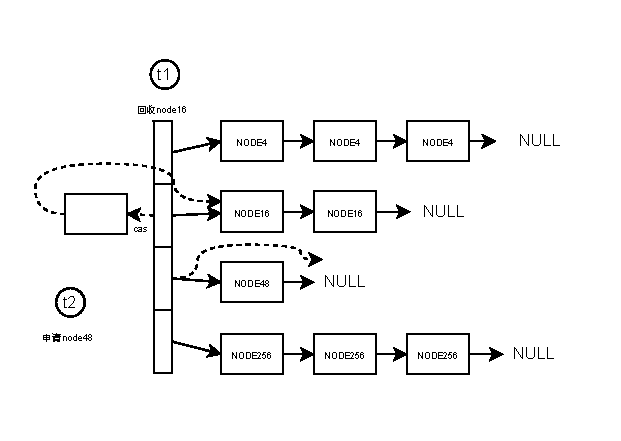
\includegraphics[width=0.6\textwidth]{art-obj-pool.pdf}
  \caption{基于无锁队列的垃圾回收}
  \label{fig:art-obj-pool}
\end{figure}

索引内存模块的空闲队列结构如上图,通常情况下,索引申请新的结点总是先从内存管理
器获取,如果内存管理器中该节点类型的空闲链表上没有空闲结点就使用 malloc 从系统申请。
当结点被标记删除时,不是立即归还给操作系统,而是将结点中 delete flag 标记为 1,同时将结
点插入到空闲队列的队头,这一步可以使用C++ 11 中的compare\_exchange\_weak 或
compare\_exchange\_strong 实现一个无锁的队列。
将一个被标记删除的空闲 Node16 结点插入空闲链表的头部。
不立即将内存归还操作系统的原因在于当前结点被标记删除后,该结点可能还被其他读进程
所占用,其他读进程仍会继续访问该节点中数据。我们将该结点标记删除后放入空闲链表,读进
程获取结点数据之后需要验证版本号,便会发现该节点已被删除需要重新从根节点进行访问。

\subsection{基于epoch的垃圾回收机制}

上述的内存管理机制适用与当前系统使用预先分配内存的方式管理内存空间。若需要及时将不用的内存归还操作系统的话,也可以通过后台的垃圾回收线程
固定回收无锁链表里的内存块,但这一操作存在风险,因为最先回收的内存总是最新标记删除的,而且随着并发度提升,无锁链表也会成为系统的瓶颈。
因此需要提升并发度,则不能使用上述内存管理机制。下面我们介绍两种基于Epoch的垃圾内存回收机制,这两种机制也是Bw-Tree作者提出的管理Bw-tree内存的机制。

\begin{figure}[h]
  \centering
  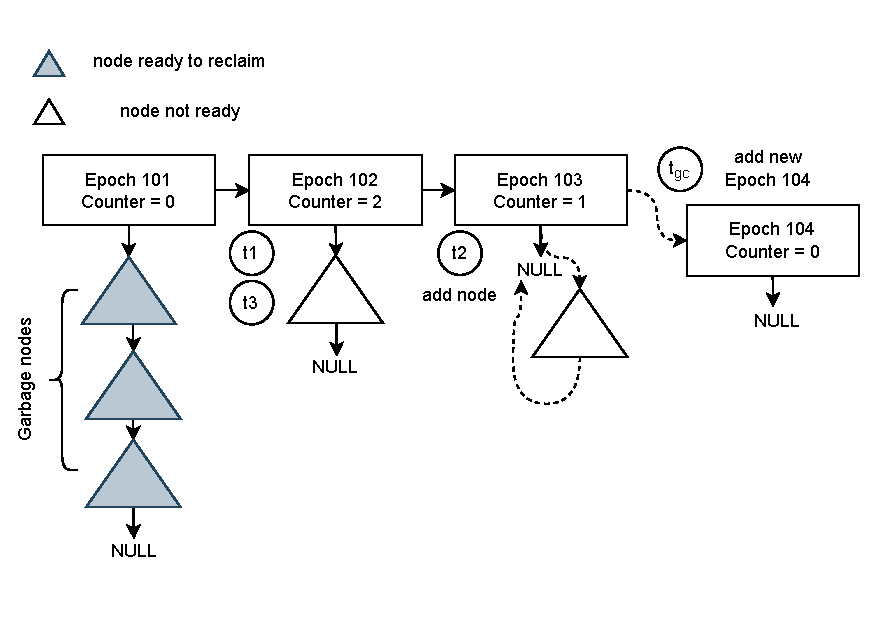
\includegraphics[width=0.7\textwidth]{art-gc-center.pdf}
  \caption{基于Epoch的中心化垃圾回收机制}
  \label{fig:art-gc-center}
\end{figure}

首先是基于Epoch的中心化的垃圾回收机制,索引维护一条全局的epoch对象链表。
后台垃圾回收线程每隔一段时间(40ms),会在链表的尾部添加一个新的epoch结构。
每个线程在访问索引内部数据结构之前,需要在当前的epoche结构中注册自己的操作,当操作完成的时候,将自己从注册过的epoch中移除
任何被标记为删除的对象都会被加入当前epoch的垃圾回收链表里。当所有的线程都离开了这个epoch,索引的垃圾回收线程会将这个epoch中
所有被标记为删除的结构回收。

上图中展示了这种中心化的垃圾回收机制。图中分别有三个工作线程和一个后台运行的垃圾回收线程。在这张图中,t2线程将一个新的节点加入
epoch103,同时垃圾回收线程新增了一个epoch104。而epoch101中的引用计数降低为0。垃圾回收线程将epoch101中所有记录的节点回收。
将其内存释放。这种垃圾回收机制的扩展性非常差,不适合作为多核多线程应用场景下使用。因为这会面临多个工作线程同时进入epoch中,同时
增加引用计数,造成资源争用。因此这会成为系统的性能瓶颈。所以以下我们讨论open-bwtree中提到另一种基于epoch的去中心化垃圾回收机制。

\begin{figure}[h]
  \centering
  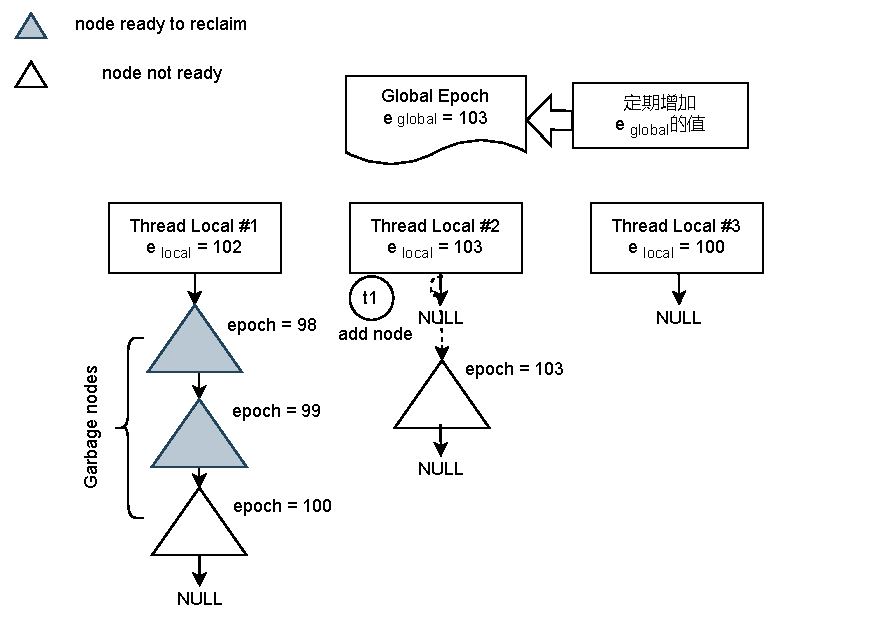
\includegraphics[width=0.7\textwidth]{art-gc-decenter.pdf}
  \caption{基于Epoch的去中心化垃圾回收机制}
  \label{fig:art-gc-decenter}
\end{figure}


上图这种去中心化的垃圾回收机制可以避免线程将数据写入到全局的内存中,从而避免多个线程并发操作导致争用问题。
下面我们详细阐述一下关于去中心化垃圾回收机制的设计。索引模块维护一个全局的epoch,每个工作线程也会维护一个本地的epoch和一个指针链表,
链表中的元素指向的是线程标记删除的对象。
还是继续使用以下的例子举例。t1作为唯一的工作线程,他将一个垃圾节点放入自己维护的链表中,并且将该节点标记为当前的epoch103。
在某个操作开始之前,线程总是先去全局的epoch拷贝一份标记删除的链表备份到自己私有的epoch中。
在进行任何操作之前,工作线程总是先从全局的epoch中读取最新的epoch存入自己的私有epoch中,此后如果该工作线程需要删除某个节点,
则将该节点标记为删除,同时将该节点标记上工作线程当前的epoch并放入自己私有的待删除链表中。

当该工作线程的工作结束之后,线程遍历所有其他工作线程的本地epoch找出最小的epoch,同时搜索本地私有链表中需要删除节点上标记小于该epoch的节点,将内存回收给操作系统。
而为了推进这个操作的可持续性,DBMS会维护一个后台线程定期增加全局的epoch。

综合以上的论述,详细阐述了如何设计基于epoch的去中心化的垃圾回收模块。其目的还是在于提高cache的命中率,期望通过读而不是写的方式可以完成线程间的同步。
使用ThreadLocal这一机制,避免了使用锁或者其他同步机制。为了方便进行编码,后面实现章节我们将借助于Intel现有的ThreadLocal库来进行操作。
后面的实现章节我们会在索引模块中分别实现两种垃圾回收机制。在实验章节,我们会对比这两种垃圾回收机制,在各种使用场景下的性能对比,
最后我们选择在不同的场景下,应当是使用不同类型的垃圾回收机制。

\section{索引主要操作流程}
这里我们介绍本章的重点就是对ART索引的并发控制,我们需要注意这里介绍的只是对ART这一数据结构的并发控制,
即同时对索引进行读写操作并不会影响数据的正确性,
关于数据库中事务的并发控制,我们将在下面小节作简单介绍,如何应用当前数据库中的事务机制做到对索引的DDL操作和DML操作也可以并发操作而不影响正确性。、
在本小节中我们主要介绍索引的查找,插入,删除,范围查找。

\subsection{查询流程}
ART索引的查询流程如上图所示,查询过程是一个只读的过程因此并不涉及到内存的申请或者释放。具体的查询流程为:

1.初始化操作:将根节点作为当作当前节点。

2.读取当前节点的版本号。

3.比较当前节点的前缀是否与需要查询的key匹配,如果匹配进入下一步骤4,如果不匹配则结束查询,返回空值。

4.当前缀匹配时,需要读取对应的槽位上是否包含子节点,如果包含子节点且为叶节点则返回其值;
若不为叶节点,则转到步骤5。

5.校验此时版本号与步骤2中的版本号是否一致,若一致说明此期间该节点没有被修改。
将非叶子节点指针读取出来赋值到当前的节点,回到步骤2进行操作。由于树形结构的深度有限,
读操作总是会读取到值或者没有匹配的值而结束这一循环。

\subsection{插入流程}
ART 索引的插入流程如上图所示,插入流程涉及到节点的扩容和新增,因此需要与内存模块交互,同时因为需要有扩容操作,涉及到将
旧的节点标记删除。

\paragraph{插入流程}
1.初始化操作:将当前节点置为空指针,将next节点置为根节点。

2.将当前节点赋值给父亲节点,next节点赋值给当前节点,读取当前节点的版本号。

3.比较当前节点的前缀是否与需要查询的key匹配,如果匹配进入第4步,如果不匹配则进入第6步。

4.验证当前节点的版本号是否与第2步读取到的一致,若一致则进入第5步,若不一致则返回第1步。

5.检查对应的槽位上是否有子节点,若含有子节点则将对应槽位上的子节点指针赋值给next指针,返回第2步,重复流程。
若对应槽位上子节点指针为空则升级当前节点和父亲节点的锁为写锁,若升级锁成功则插入新的节点;若升级锁失败,返回第1步重试。
在这里需要注意的是插入可能会导致节点类型升级,所以也需要升级父亲节点的锁为写锁。

6.当前节点的前缀与插入的key不匹配。首先获取父节点的锁,然后获取当前节点的写锁。
若有一个失败,则返回第1步重试。再次取出取出两者的公共部分,申请一个新的Node4类型的节点,
将当前节点和需要插入的节点分别插入其中对应位置。将父结点中对应的子节点指针修改为新申请的Node4节点的地址,完成插入流程。

\subsection{范围查询流程}
范围查询是索引中经常使用的一种查询方式,比如select * form tb where idx < 1000 and idx > 200,
且idx字段为索引字段。ART索引的范围查询流程如下所示。

1.初始化操作:将根节点作为当作当前节点。

2.读取当前节点的版本号。

3.比较当前节点的前缀与startKey和endKey的大小关系,若startKey大于当前前缀或者endKey小于当前前缀,说明不存在有效的结果。
此时应当验证版本号,若与步骤2中的一致,返回空集;若不一致,则返回第一步中的根节点重新查找。

4. 若当前的前缀恰好在闭区间startKey和endKey之间(此处应当是严格小于endKey[level],严格大于startKey[level],level表示此时在键值中的位置),
验证版本号若一致,则将当前节点下所有的叶子节点存储Tid加入结果集,返回结果;若不一致,返回第一步重新开始查询。
若前缀恰好可以完全匹配当前的区间要求,则读取当前节点上的所有满足闭区间[startKey[level+1], endKey[level+1]]的子节点指针。
针对边界值,使用递归进行查询,以区间的起始位置举例,查询的范围变为[startKey, 无穷大值],同理针对区间的结束位置,查询范围变成了
[无穷小值, endKey]。因为ART树的内部节点键值的取值范围为0至255,因此这里的无穷大,无穷小对应的分别就是全部字节皆为255和0的
键值。而针对非边界的子节点指针,查询的方式类似于前面的前缀恰好严格落在查询区间中的方式。
最终我们返回的是三者的并集。

\subsection{删除流程}
删除流程大致与插入流程类似,区别在于删除节点可能会导致节点收缩,当子节点的个数低于阈值时,需要将容量较高的节点缩减为下一级
容量的节点,这里我们需要修改父节点中对应的指向子节点的指针,同时需要将原来节点中的子节点拷贝到新的节点中,并将原节点标记删除。
以下为详细的流程设计:
\paragraph{删除流程}
1.将根节点作为当前节点。

2.读取当前节点的版本号。

3.比较当前节点的前缀是否与需要查询的key匹配,如果匹配进入第4步,如果不匹配则直接返回。

4.验证当前节点的版本号是否与第2步一致,若一致则进入第5步,若不一致则返回第1步。

5.检查对应的槽位上子节点是否为空指针,若对应的子节点不为空且不是叶子节点则将当前节点替代为子节点,返回第2步,继续向下搜索。
若对应的子节点指针不为空且为叶子节点则升级当前的节点与父亲节点的锁等级,删除对应的叶子节点。这里升级父亲节点的锁等级的目的在于
当前节点删除一个子节点指针之后会不满足当前节点类型的最低子节点个数的要求。因此这里需要申请更小类型的索引节点,并将父亲节点
中的对应子节点指针修改为新申请的节点。

\section{不同类型数据的键值设计}
我们知道在数据库系统中存在着许多不同的种类,在类型上大体可以分为变长和定长,索引需要向外提供范围查询功能,因此实际上
存储的数据应当是有序的,这样会方便我们进行范围查询。
而由于ART树的特殊性,每个节点只存储部分索引的字段,所以合理的安排索引的顺序就显得非常重要了。
由于前缀树的设计,我们需要对不同类型的数据做出适当的变换以适应前缀树的存储方式。
以下我们重点介绍int/uint, float/double,String,复合的key。

\subsection{int/uint的存储结构设计}
对于unsigned类型其对应的二进制类型仍具有既定的顺序,但是我们仍然需要考虑到大小端的问题。
因此对于小端系统,我们需要将字节序反转以保证结果是有序的。而如何判断系统属于大端还是小端系统,可以在系统中定义相关的宏,
编译器根据指定平台的编译出相应的代码。

而对于signed类型,则需要重新排序,因为负数在计算机中按照补码存储,
一个b位的整数x可以通过反转符号位转换为正常的顺序(x XOR $2^b$-1),变换后有符号数就可以按照无符号树的顺序进行比较,
随后就可以作为正常的无符号进行存储。

\subsection{float/double的存储结构设计}
首先对于IEEE754类型的浮点数,可以优先根据符号位将其区分为整数和负数,
其次可以将其分为规格化的值,非规格化的值,NaN,无穷大/小,0。总计十种数值。
他们彼此之间是没有交集的。因此只需要将阶码,尾数转换为对应的无符号数处理即可

以double类型举例,考虑其13位的阶码和52位的尾数,分别使用2字节和9字节存储。最高为符号,因此这样的话root节点只需要作为
一个Node4类型的节点存储两个key指向的孩子节点。

\subsection{string的存储结构设计}
对于string类型的处理分为两种,一种较为简单针对定长的string类型,我们可以简单的将其对齐到指定的字节数(128bytes,256bytes,512bytes)。对于空出来的位数可以直接填0。
对于不定长的string类型,这种数据类型主要的使用场景是支持LPM(最长前缀匹配),
这需要我们修改原本的数据结构,即在node header中加入一个判断条件支持多增加的这一对(key/value),当进行前缀比较时,需要注意这一点,
因为原始的ART中是不存在前缀特征的键值的,而这里加入前缀特征之后,每一个节点的孩子节点的容量都会增加1,而且为了支持最长前缀匹配,当搜索key时
需要作出特殊处理。这在后续的支持LPM匹配的查询处做详细说明。
通常情况下我们所存储的key均为定长数据,因此不会产生这种一个键值是另一个键值的前缀的场景。

\subsection{compound key的存储结构设计}
对于复合类型的key,通常情况下,生成索引部分需要传入组合键值的相应参数,IndexBuilder根据参数生成相应的索引结构。
因此只需要在传入参数时,根据上述介绍的规则逐个转换,选择合适大小的索引类型生成即可。

我们需要注意的是本索引并不允许两个重名的字段出现,即需要索引的字段应该是全局唯一的,但是实际上许多字段并不能做到全局唯一,
因此,我们需要在判断字段是否相同时,加入该字段的唯一主键,这个主键可以是记录的TID。以上便可以做到全局索引到唯一的一条记录。

\section{事务机制}
上述介绍的索引模块中引入的并发控制机制仅仅是针对该数据结构的并发控制,全部为DML操作,还有一类比较特殊的操作例如
create/drop index操作。

针对创建索引的操作,索引模块主要接口为根据keySchema创建相应的索引,这里主要是根据keySchema确定ART索引中键值的长度。
根据以上小节提到的针对不同数据类型所需要作出的更改。

针对需要删除索引的操作,这里有两个地方需要注意。一个是当索引模块需要删除该索引时,可能还有其他事务的进程在读取该索引,
所以我们并不能直接删除索引,而是利用一种叫做DAF事务框架的方式,作延迟删除。详细的如何延迟删除在下一小节讲解。
另一个需要注意的地方是需要删除所有索引的内存,如果索引采取的预先分配内存的方式,那么直接回收内存即可。如果采用的
是基于Epoch的垃圾回收机制,则需要从根节点开始,以类似于后序遍历的方式,逐个回收节点内存,由于采用的是去中心化的垃圾回收机制。
随着最后一个操作结束,如果此时操作退出时没有能够回收已经标记删除的内存,那这块内存会一直保留着。
因此基于Epoch的垃圾回收机制还需要注意在清理对象时,回收掉没能立即被回收的内存块。

\subsection{DAF的基本结构设计}
DAF事务框架(Deferred Action Framework)核心在于
如何将事务性的修改(删除索引中的一条记录)和非事务性的修改(删除索引)结合。
框架的核心在于将所有对实际物理结构上的操作都注册为一个action,
数据库系统针对不同的命令会执行对应的action, 但是这些action真正的执行需要等到系统安全为止。
直到该版本不再被当前活动的事务可见时管理器就会删除这个版本。

\subsection{DAF事务框架}

\begin{figure}[h]
  \centering
  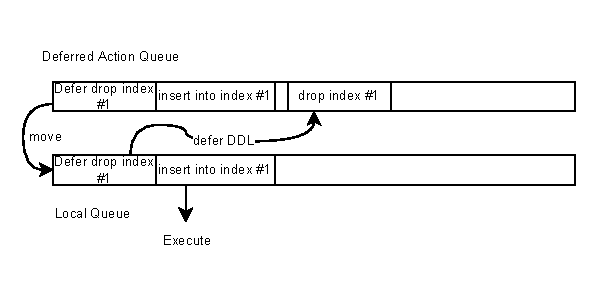
\includegraphics[width=0.7\textwidth]{daf.pdf}
  \caption{DAF 延迟删除}
  \label{fig:daf}
\end{figure}

由于DAF事务框架的设计规定,我们在整个系统设计一个DAF Manager,
他负责管理事务延期执行的行为。主要设计思路是维护一个队列,队列里的元素为Deferred Action,
而Deferred Action则为对应的一个个动作。如上图,当索引需要删除时,将这个删除索引的操作,注册到
DAF Manager中,这个操作实际上注册是延迟删除索引的操作,因此当DAF Manager 执行以下队列的操作时,尽管删除索引的
操作在对索引执行插入操作之前,但是实际上,DAF Manager只会将该drop index 操作再次注册进队列中,等待下次执行队列的机会。
而且在执行Deferred Action时可以执行并发操作,因为此时所有需要删除的记录都是对当前事务不可见的。

这里的事务框架是系统中已有的事务框架,我们这里只是简单介绍其与索引模块相关的操作。

\section{底层存储机制设计}
上述章节已经介绍了索引设计和如何将索引引入数据库中。
下面我们再介绍一下底层存储模块即表存储设计,
由于本索引应用于内存数据库即所有的数据都存储在内存上因此没有传统数据库中的buffer pool的概念,
但是我们仍然需要建立对内存块的维护,并且设计新的内存存储系统。

\subsection{底层存储组织格式}
传统的数据库往往根据其主要的使用场景将其分为OLAP和OLTP,
针对OLTP数据库来说,其往往会采用行式来组织数据,
而OLAP数据库会采用列式组织数据,这两种数据组织方式各有其优缺点。
而我们采取的是行列混存方式,同时还可以引入冷热数据分开存储的方式,
将冷数据转换为Arrow的纯列式存储,不仅方便数据后期的分析查询,还可以提供通用接口供其他应用调用。

\subsection{PAX行列混存格式设计}

\begin{figure}[h]
  \centering
  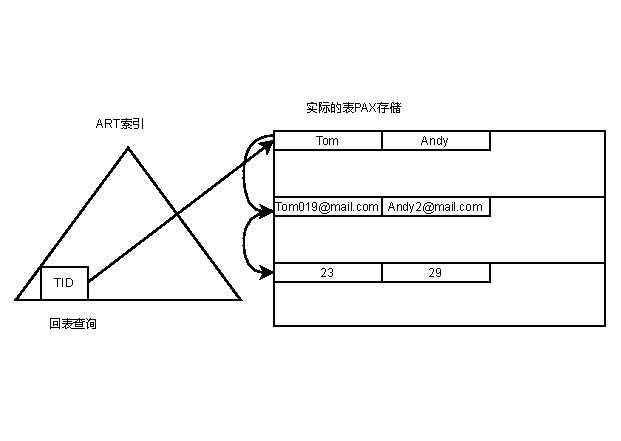
\includegraphics[width=0.7\textwidth]{art-table-pax.pdf}
  \caption{PAX行列混存格式}
  \label{fig:art-table-pax}
\end{figure}

行列混存格式,即将整个数据分成合适大小的block,在block之间采用行存方式组织数据,
但是在block内部采用列存。block内部根据该表的所存储记录的metadata,将每一个block划分为多个miniblock
每个miniblock的大小根据metaData计算出来,因此所有的miniblock的大小在插入数据之前就已经确认了。所以实际block的存储
记录中不可以含有变长记录。这点可以通过超过指定长度的变长数据就通过指针方式存储。
而且由于是内存数据库,因此每个block可以根据指针直接访问。每个block内部的数据组织格式如下图所示。
这里主要是提出对变长信息的优化,由系统维护一个var entry 管理器,超过16字节的变量就由varlen负责存储。
采用前8字节为长度,后8字节为变量的地址。即可寻址到具体的变长变量。
同时这里也可以做到一个如果实际存储的字段的基数较低,可以部分存储字段,而不用完全存储。
通过低基数优化还可以同时优化字段作为聚合字段时的开销。
上文中提到ART索引,作为系统中的辅助索引,其每一个叶子节点均指向实际的内存地址(即图中所示的version ptr)。
由于正常的linux系统中,虚拟地址只需要前48位,因此我们可以将最高位置为1的方式,来区分叶子节点和实际的虚拟地址空间。

这样,我们在索引的叶子节点中只需要存储TupleId,即存储一个64位的地址。通过这个地址,再去内存的表中读取相应的记录。

\subsection{Apache Arrow存储格式}
由于系统中存在两种数据组织格式,冷数据以Apache Arrow\cite{ahmad2020arrowsam}格式组织,方便其他应用直接获取。
Apache Arrow 是一种跨平台跨语言的内存列式数据组织格式。
在Apache出现之前,每个系统之间互相传输数据都需要经过序列化和反序列化,在系统数据量较大的情况下,大量计算资源消耗在上面,这无疑造成了系统的开销。
Arrow数据组织上严格按照字节对齐,最大化利用硬件带来的向量化和SIMD加速。其将数据分为两类,定长和变长数据类型,并使用Array表示。定长Array包括
数据类型,长度,空值个数,空值位图,按字节组织的列数据。
变长与定长组织方式类似,但是会多一个数据偏移字段,以帮助数据快速定位和计算长度。

因此内存索引中如何索引这些按照Arrow格式组织的冷数据。
可以建立一个对于冷数据的管理器,根据TID的标记到这个管理器中查询对应的记录。由于Arrow格式本身
也可以持久化到磁盘中,因此如果系统开启了冷热数据分区的话。
对于冷数据的索引就会退化为面向磁盘的数据库索引,因此已经不再适合当前的索引类型。所以本文只讨论
所有需要索引的记录均存储在内存中。

总的来说,目前ART索引只适合索引那些存储在内存上的数据,如果涉及到需要与磁盘交互的部分,那么索引的很多设计思路就失效了。
因此ART索引只适合作为内存数据库索引而被使用。

\section{本章小结}
本章先介绍了基于乐观锁的ART的诞生背景以及明确索引设计的目标,对索引的各个部分的设计和流程进行了简要介绍。
首先是索引node中各个参数的内存分布,以及如何基于原子变量实现乐观锁,
其次介绍了级联锁即每个并发操作只会同时拥有两把锁。
针对并发操作中可能产生的内存回收问题,设计无锁队列回收内存,并重复使用该内存,降低了系统调用的开销。但是以上这种方式仅适用于
预先分配内存的情况。针对不预先分配内存,实时申请释放内存的系统,采用基于Epoch的垃圾回收机制。
然后我们逐个介绍了索引的点查询,删除,插入,范围查询等流程。
最后两小节中,我们介绍如何将数据库索引的DDL操作与DML操作都融入数据库的事务系统中,但这部分并不是本文讨论的重点。
此外我们还介绍了实际数据库系统中表的存储结构采用PAX的存储方式,通过TupleID 访问一条记录需要跨过多个miniBlock,
因此这里我们就不再对索引进行路径压缩,在路径上保留完整的key,只通过公共前缀的方式进行数据压缩。
